\documentclass[12pt]{article}
\usepackage{anyfontsize}
\usepackage[margin =2cm]{geometry}
\usepackage{polski}
\usepackage[utf8]{inputenc}
\usepackage{titlesec}
\titlelabel{\thetitle.\quad} 
\usepackage{tabto}
\usepackage{graphicx}
\usepackage{amsmath}
\usepackage{multicol}
\usepackage{mathtools}

\usepackage{csvsimple}
\usepackage{pgfplots}

\usepackage[european, americanvoltages, RPvoltages]{circuitikz}
\usepackage{tikz}

\title{\underline{Wzory, równania i zależności}\\\textbf{z teorii sygnałów}}
\author{Łukasz Przystupa}
\date{\today}
\pgfplotsset{compat=1.18}

\usepackage{titling}
\renewcommand\maketitlehooka{\null\mbox{}\vfill}
\renewcommand\maketitlehookd{\vfill\null}


\DeclareMathOperator{\FT}{\xleftrightarrow[\text{ICFT}]{\text{CFT}}}
\DeclareMathOperator{\CFT}{\xleftrightarrow[]{\text{CFT}}}
\DeclareMathOperator{\ICFT}{\xleftrightarrow[\text{ICFT}]{}}

\begin{document}

    \maketitle
    całość opara na wykładach Kohorty i Sypki.
    \newpage

    \section{Wzory Eulera}
% 
\begin{multicols}{2}
    \begin{gather*}
        e^{jx} = \cos{(x)} + j\sin{(x)}\\
        \sin{(x)} = \frac{e^{jx}-e^{-jx}}{2j}\\
        \cos{(x)} = \frac{e^{jx}+e^{-jx}}{2}\\\\
        % 
        \cosh{(x)} = \frac{e^x+e^{-x}}{2}
    \end{gather*}

    \begin{gather*}
        \sin{(\alpha+\beta)} = \sin{(\alpha)}\cos{(\beta)} + \cos{(\alpha)}\sin{(\beta)}\\
        \sin{(\alpha-\beta)} = \sin{(\alpha)}\cos{(\beta)} - \cos{(\alpha)}\sin{(\beta)}\\
        % 
        \cos{(\alpha+\beta)} = \cos{(\alpha)}\cos{(\beta)} - \sin{(\alpha)}\sin{(\beta)}\\
        \cos{(\alpha-\beta)} = \cos{(\alpha)}\cos{(\beta)} + \sin{(\alpha)}\sin{(\beta)}
        \\\\
        \sinh{(x)}=\frac{e^x-e^{-x}}{2}
    \end{gather*}
\end{multicols}


\section{Sygnał jako wektor}
    Iloczyn skalarny:
    \begin{equation*}
        <x, y> = \int\limits_{D} x(t) \cdot \overline{y(t)} dt
    \end{equation*}
    Norma (długość wektora):
    \begin{equation*}
        ||x(t)||^2 = <x(t), x(t)>
    \end{equation*}
    Metryka (odległość sygnałów):
    \begin{equation*}
        \rho(x,y) = ||x-t|| = \sqrt{<x(t)-y(t), x(t)-y(t)>}
    \end{equation*}

    \noindent
    Korelacja (jak bardzo sygnały są podobne):
    \begin{equation*}
        R_{xy}(t) = \int\limits_{-\infty}^{+\infty}x(\tau)\cdot \overline{x(\tau-t)}\ d\tau
    \end{equation*}

    \noindent
    Energia sygnału:
    \begin{equation*}
        Energia(x(t)) = ||X(t)||^2_{L^2} = \int\limits_D |x(t)|^2dt
    \end{equation*}

    \noindent
    Wektory są ortogonalne (czyli prostopadłe względem siebie (czyli liniowo niezależne)) jeśli:
    \begin{equation*}
        <x(t), y(t)> = ||x(t)|| \cdot ||y(t)|| \cdot cos(\alpha) = 0 \Leftrightarrow x\perp y
    \end{equation*}


    \subsection{Twierdzenie Percevala - o zachowaniu energii}
        \begin{gather*}
            \int\limits^{+\infty}_{-\infty}|x(t)|^2 dt\ = \int\limits^{+\infty}_{-\infty}|X(f)|^2df
        \end{gather*}
    \subsection{Twierdzenie o zmianie skali}
        \begin{gather*}
            \delta(a\cdot t) \FT \frac{1}{|a|}\cdot\delta(f)
        \end{gather*}
    \subsection{Twierdzenie o zachowaniu odległości}
        Jeżeli:
        \begin{gather*}
            x(t)\circ y(t) \FT X(f)\circ Y(f)
        \end{gather*}
        to:
        \begin{gather*}
            ||x(t) - y(t)|| = ||X(f) - Y(f)||
        \end{gather*}

    \subsection{Splot}
        Definicja:
        \begin{gather*}
            y(t) = \int \limits _{-\infty}^{+\infty}x_1(\tau) x_2(t-\tau) \,d\tau\\
            y(t) = x_1(t)*x_2(t) 
        \end{gather*}

        \noindent
        Właściwości splotu:
        \begin{gather*}
            x_1(t)*x_2(t)\xleftrightarrow[ICFT]{CFT} X_1(f)X_2(f)\\
            x(t)*\delta(t-t_0) = x(t-t0)
        \end{gather*}
    \section{Szereg Fouriera}
    Postać numeryczna:
    \begin{gather*}
        x_F = a_0 + \sum\limits_{n=-\infty}^{+\infty}a_n\cdot cos\left(2\pi n\right) +b_n\cdot sin\left(2\pi n\right)
    \end{gather*}

    \indent Postać okresowa:
    \begin{align*}
        c_n = \frac{1}{T}\cdot \int\limits_{t_0}^{t_0+T}x(t) && gdzie:\ T - okres\ x(t)\\
% 
        x(t) = \sum\limits_{n=-\infty}^{+\infty}c_n\cdot e^{+j2\pi nf_T t} && gdzie:\ f_T = 1/T 
    \end{align*}
    Sygnał musi spełniać warunki Dirichleta!!!


\section{Definicje różnych transformat}
    \subsection{Transformata Fouriera (CFT i ICFT)}
        \begin{multicols}{2}
            \begin{gather*}
                x(t) \xleftrightarrow[\text{aaa}]{\text{bbb}} X(f)\\
                X(f) = \int\limits_{-\infty}^{+\infty} x(t) e^{-j2\pi f t}  \,dt 
            \end{gather*}

            \begin{gather*}
                x(a t)\xleftrightarrow[\text{ICFT}]{\text{CFT}} \frac{1}{|a|} X(\frac{f}{a})\\
                x(t - t_0)\xleftrightarrow[\text{ICFT}]{\text{CFT}} X(f)e^{-2j\pi ft_0}\\
                \overline{x(t)} \xleftrightarrow[ICFT]{CFT} \overline{X(-f)}
            \end{gather*}
        \end{multicols}
        Należy wspomnieć że iloczyn skalarny jest niezależny od wybranej dziedziny:
        \begin{gather*}
            x(t)\circ(y) \xleftrightarrow[\text{ICFT}]{\text{CFT}} X(f) \circ Y(t)\\
            \Downarrow\\
            \int\limits^{+\infty}_{-\infty}x(t)\overline{y(t)} dt \ \textbf{=} \int\limits^{+\infty}_{-\infty}X(f)\overline{Y(f)}df
        \end{gather*}


    \subsection{Transformacja sygnału próbkowanego}
        \begin{gather*}
            x_p(t) = x(t)\cdot g_{\Delta t}(t) = \sum_{n=-\infty}^{+\infty}x(n\Delta t)\cdot\delta(t-\Delta t)\\
            \Downarrow\\
            X_p(f) = X(f) * G_{\Delta t}(f) = X(f) * \left[\frac{1}{\Delta t} \sum_{n=-\infty}^{+\infty}\delta(f-n\cdot f_p)\right]
        \end{gather*}

    \subsection{Transformacja Dyskretna (DTFT)}
         \begin{multicols}{2}
            \begin{gather*}
                x_p = \sum\limits_{n=-\infty}^{+\infty}x(n\Delta t)\cdot \delta(t-n\Delta t)
            \end{gather*}

            \begin{gather*}
                X(f) = \sum\limits_{n = -\infty}^{+\infty}x(n\Delta t) \cdot e^{-j2 \pi \frac{f}{f_{p}}\cdot n}\\
                gdzie:\ f_p =\ f\ probkowania
            \end{gather*}
         \end{multicols}

    \subsection{Transformacja Hilberta}
        \begin{multicols}{2}
            \begin{gather*}
                x(t) \xleftrightarrow[\text{IHT}]{HT} x^H(t)\\
                x^H(t) = -\frac{1}{\pi}  \cdot \int\limits_{-\infty}^{+\infty}\frac{x(\tau)}{\tau-t}\ d\tau
            \end{gather*}

            \indent Czyli:
            \begin{gather*}
                x^H(t) = \frac{1}{\pi\cdot t}*x(t) = h_H(t)*x(t)\\
                \Downarrow\\
                h_H(t) \FT -j \cdot sgn(f)
            \end{gather*}
        \end{multicols}
    % \newpage

        

    % \newpage
\section{Sygnały podstawowe i ich transformaty}
    \begin{multicols}{2}
        \begin{gather*}
            x(t) = \sin{(2\pi ft)}\\
            x(t) = \cos{(2\pi ft)}\\
\\% 
            \Pi(t) = \left\{\begin{array}{l l}
                1 & dla\ |t| < 1/2\\
                1/2 & dla\ |t| = 1/2\\
                0 & dla\ |t| > 1/2
            \end{array} \right.\\
\\%  
            sinc(t) = \left\{\begin{array}{l l}
                \frac{\sin{(2\pi f)}}{2\pi f} & dla\ t \neq 1\\
                1 &\ dla\ t = 0
            \end{array}\right.\\
\\% 
            \Lambda(t) = \left\{\begin{array}{l l}
                t+1 & dla\ -1 \leq t \leq 0\\
                -t+1 & dla\ 0 < t \leq 1\\
                0 & dla\ pozostalych\ t
            \end{array}\right.\\
\\%
            u(t) = \left\{\begin{array}{l l}
                1 & dla\ t>0\\
                \frac{1}{2} & dla\ t=0\\
                0 & dla\ t <0
            \end{array}\right.
\\%
            sgn(t) = \left\{\begin{array}{l l}
                1 & dla\ t>0\\
                \frac{1}{2} & dla\ t=0\\
                -1 & dla\ t <0
            \end{array}\right.
        \end{gather*}


        \begin{gather*}
            \cos{(x)} \xleftrightarrow[ICFT]{CFT} \frac{1}{2}(\delta(f+f_0) + \delta(f-f_0))\\
            \sin{(x)} \xleftrightarrow[ICFT]{CFT} j\frac{1}{2}(\delta(f+f_0) + \delta(f-f_0))\\\\
            \delta(x) \xleftrightarrow[ICFT]{CFT} 1\\\\
            \Pi(t) \xleftrightarrow[\text{ICFT}]{\text{CFT}} sinc(\pi f)\\\\
            \Lambda(x) \xleftrightarrow[ICFT]{CFT} sinc^2(\pi f)\\\\
            g_T(t) = \sum \frac{1}{T} e^{j2\pi f_n t} \xleftrightarrow[ICFT]{CFT} G_T(f) = \sum \delta(f-\frac{n}{T})\\\\
            u(t) \FT \frac{1}{2}\delta(f) + \left\{\begin{array}{l l}
                -j\cdot\frac{1}{2\pi f} & dla\ f\ne 0\\
                0 & dla\ f=0
            \end{array}\right.\\
            sgn(t) \FT \left\{\begin{array}{l l}
                -j\cdot\frac{1}{2\pi f} & dla\ f\ne0\\
                0 & dla\ f=0
            \end{array}\right.
        \end{gather*}
    \end{multicols}


% \subsection*{Twierdzenia pomocniczne}
%     \begin{gather*}
%         x(t)\xleftrightarrow[ICFT]{CFT}X(f)\\
%         \overline{x(t)}\xleftrightarrow[ICFT]{CFT}\overline{X(-f)}\\
%         % Do przemyślenia
%         % x(t)\xleftrightarrow[ICFT]{CFT} \frac{1}{2\pi}X(\omega)
%     \end{gather*}
    \section{Sygnały okresowe:}
    \begin{align*}
        x(t) = x(t+n\cdot T) && Gdzie:\ T- okres\ podstawowy\\
        n = ...-2, -1, 0, 1, 2...
    \end{align*}
    \begin{equation*}
        x(t) = \sum_{n = -\infty}^{+\infty}x_0(t-n\cot T)
    \end{equation*}
    Gdzie $x_0(t)$ - wzorzec sygnału,

    \begin{equation*}
        x(t) = \sum_{n=-\infty}^{+\infty}x_0(t-n\cdot T) = x_0(t) * \sum_{n=-\infty}^{+\infty}\delta(t-n\cdot T) = x_0(t)*g_T(t)
    \end{equation*}
    Fukcja $g_T(t)$ jest to pseudo fukcja reprezentująca grzbień Diraca

    \subsection*{Dla fukcji zepolonych:}
        \begin{align*}
            x(t) = \sum_{n=-\infty}^{+\infty} c_n \cdot e^{j2\pi n f_T t} && f_t = \frac{1}{T}\\
            c_n = \frac{1}{T} \int\limits_{-T/2}^{+T/2} x(t)\cdot e^{-j2\pi f_nt}dt && f_n = n\cdot f_T
        \end{align*}
    \section{Sygnał jako wektor}
    Iloczyn skalarny:
    \begin{equation*}
        <x, y> = \int\limits_{D} x(t) \cdot \overline{y(t)} dt
    \end{equation*}
    Norma (długość wektora):
    \begin{equation*}
        ||x(t)||^2 = <x(t), x(t)>
    \end{equation*}
    Metryka (odległość sygnałów):
    \begin{equation*}
        \rho(x,y) = ||x-t|| = \sqrt{<x(t)-y(t), x(t)-y(t)>}
    \end{equation*}

    Energia sygnału:
    \begin{equation*}
        Energia(x(t)) = ||X(t)||^2_{L^2} = \int\limits_D |x(t)|^2dt
    \end{equation*}

    Wektory są orogonalne (czyli prostopadłem względem siebie (czyli liniowo niezależne)) jeśli:
    \begin{equation*}
        <x(t), y(t)> = ||x(t)|| \cdot ||y(t)|| \cdot cos(\alpha) = 0 \Leftrightarrow x\perp y
    \end{equation*}


    \subsection{Twierdzenie Persevala - o zachowaniu energii}
        \begin{gather*}
            \int\limits^{+\infty}_{-\infty}|x(t)|^2 dt\ = \int\limits^{+\infty}_{-\infty}|X(f)|^2df
        \end{gather*}
    \subsection{Twierdzenie o zachowaniu odległości}
        Jeżeli:
        \begin{gather*}
            x(t)\circ y(t) \FT X(f)\circ Y(f)
        \end{gather*}
        to:
        \begin{gather*}
            ||x(t) - y(t)|| = ||X(f) - Y(f)||
        \end{gather*}

\section{Aproksymacja syngału}
    Aproksymacją sygnału $x(t)$ jest:
    \begin{equation*}
        x(t) \approx \sum_{n=1}^{N}a_nb_n(t)
    \end{equation*}
    czyli:
    \begin{align*}
        x(t)  \textbf{+}e(t) = \sum_{n=1}^{N}a_n\cdot b_n(t)\\
        x(t) = \sum_{n=1}^{N}a_n\cdot b_n-e(t)
    \end{align*}
    gdzie współczynniki $a$ i $b$ odpowiadaja macioerzom:
    \begin{align*}
        b = A \cdot a\\
        % 
        b = \left[\begin{array}{c}
            x\circ b_1\\
            x\circ b_2\\
            x\circ b_3\\
            ...\\
            x\circ b_N
        \end{array}\right] &&
        A = \left[\begin{array}{c c c c}
            b_1\circ b_1 & b_2\circ b_1 & ... & b_N\circ b_1\\
            b_1\circ b_2 & b_2\circ b_2 & ... & b_N\circ b_2\\
            b_1\circ b_3 & b_2\circ b_3 & ... & b_N\circ b_3\\
            ...          & ...          & ... & ...\\
            b_1\circ b_N & b_2\circ b_N & ... & b_N\circ b_N
        \end{array}\right] &&
        a = \left[\begin{array}{c}
            a_1\\
            a_2\\
            a_3\\
            ...\\
            a_N
        \end{array}\right]
    \end{align*}

    W gdyby wektorty byłyby ortogonalne, całość sprowadza się do prostego równania:
    \begin{align*}
        a_k = \frac{x\circ b_k}{||b_k||^2} && k = 1, 2, ..., N
    \end{align*}

    Kiedy nasze wektory są znormalizowane to:
    \begin{align*}
        ||b_k||^2 = 1\\
        a_k = x\circ b_k  && k = 1, 2, ..., N
    \end{align*}
    
\section{Baza Harra (ortonormalna)}
    \begin{align*}
        H_{0,0}(t) = \Pi(t-0.5) && D: t\in <0, 1>\\
        H_{0,1} = \Pi(2\cot(t-0.25))-\Pi(2\cdot(t-0.75))\\
        H_{k,m} = 2^{\frac{k}{2}}\cdot H(2^k\cdot (t-\frac{m-1}{2^k})) && m = 1, 2, ..., 2^k
    \end{align*}

    \begin{multicols}{2}
        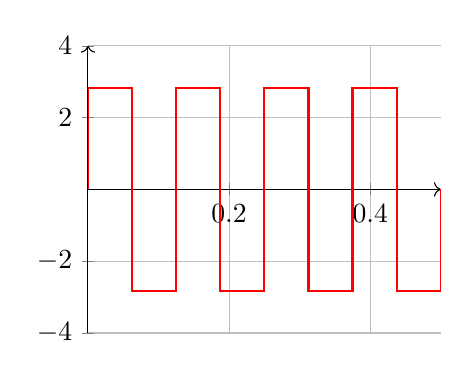
\begin{tikzpicture}
            \begin{axis}[
                width =0.5\textwidth,
                xmajorgrids = true,
                ymajorgrids = true,
                legend style={at={(0.85, 0.25)},anchor=north,legend cell align=south east},
                axis lines=middle,
                axis line style={->},
                xmax = 0.5,
                ymin = 0,
                ymax = 4,
                ymin = -4
            ]
                \addplot[red, thick, mark=none, const plot] coordinates 
                {(0,0) (0, 2.82) (0.0625,2.82) (0.0625, -2.82) (0.125, -2.82) (0.125, 2.82) (0.1875, 2.82) (0.1875, -2.82) (0.25, -2.82) (0.25, 2.82) (0.3125, 2.82) (0.3125, -2.82) (0.375, -2.82) (0.375, 2.82) (0.4375, 2.82) (0.4375, -2.82) (0.5, -2.82) (0.5, 0)};
            \end{axis}
        \end{tikzpicture}

        Czyli kolejne sygnały bazy:
        \begin{gather*}
            b_1(t) = H_{0,0}(t)\\
            b_2(t) = H_{0,1}(t)\\
            b_3(t) = H_{1,1}(t)\\
            b_4(t) = H_{1,2}(t)\\
            b_5(t) = H_{2,1}(t)\\
            b_6(t) = H_{2,2}(t)\\
            ...
        \end{gather*}
    \end{multicols}

\section{Baza Walsha}
    \begin{align*}
        W_{0, 0}(t) = \Pi(t-0.5) && D: t\in<0, 1>\\
        W_{0, 1}(t) = W_{0, 0}(2t)+(-1)^1\cdot W_{0, 0}(2\cdot(t-0.5))\\\\
        W_{k, 2m-1}(t) = W_{k-1, m}(2t)+(-1)^{m-1}\cdot W_{k-1, m}(2\cdot(t-0.5)) && dla\ k > 1\\
        W_{k, 2m}(t)   = W_{k-1, m}(2t)+(-1)^{m}  \cdot W_{k-1, m}(2\cdot(t-0.5)) && dla\ k > 1
    \end{align*}

    \begin{multicols}{2}
        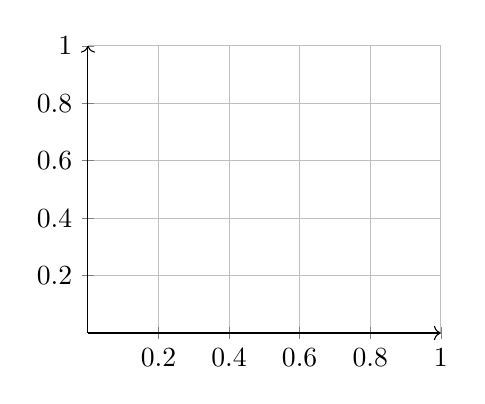
\begin{tikzpicture}
            \begin{axis}[
                width =0.5\textwidth,
                xmajorgrids = true,
                ymajorgrids = true,
                legend style={at={(0.85, 0.25)},anchor=north,legend cell align=south east},
                axis lines=middle,
                axis line style={->},
                xmax = 0.5,
                ymin = 0,
                ymax = 1.25,
                ymin = -1.25
            ]
                % \addplot[red, thick, mark=none, const plot] coordinates 
                % {(0, 0)};
            \end{axis}
        \end{tikzpicture}
        
    \end{multicols}
    \section{Twierdzenie o pochodnej}
    \subsection*{Pochodna pierwszego rzędu:}
        \begin{gather*}
            dla\ \underset{t\rightarrow\pm\infty}{lim}\ x(t) = 0\\
            \frac{d}{dt}x(t) \FT j2\pi f\cdot X(f)
        \end{gather*}
    \subsection*{Pochodna \textbf{n}-tego rzędu:}
        \begin{gather*}
            dla\ \underset{t\rightarrow\pm\infty}{lim}\ x^{(m)}(t) = 0\ :\ m = 0,1,2,...,n-1\\
            \frac{d^n}{dt^n}x(t)  \FT (j2\pi f)^{n}\cdot X(f)
        \end{gather*}

\section{Twierdzenie o całce}
    \begin{gather*}
        \int\limits^{-\infty}_{t} x(\tau)d\tau \FT \frac{1}{j2\pi f}\cdot X(f)\ dla\ f=0
    \end{gather*}
        dla $f=0$ liczymy osobno.
    
    \section{Filtry}
    Głównym parametrem określającym filtr jest jego transmitancja:
    \begin{equation*}
        H(s) = \frac{b_0\cdot s^0+b_1\cdot s^1+ b_2\cdot s^2...}{1+a_1\cdot s + a_2\cdot s^2...}
    \end{equation*}
    Transmitancje można rozłożyć na ułamki proste, tak że miejsca zerowania licznika to ,,zera" a miejsca zerowania mianownika to ,,bieguny"
    \begin{equation*}
        H(s) = \frac{b}{a}\cdot \frac{(s-z_0)\cdot(s-z_1)...}{(s-p_0)\cdot(s-p_1)...}
    \end{equation*}
    Następnie zgodnie z zasadą na rozkładanie na ułamki proste:
    \begin{equation*}
        H(s) = \frac{c_0}{s-p_0}+\frac{c_1}{s-p_1}+\frac{c_3}{s-p_3}+...
    \end{equation*}
    Z założeniem że:
    \begin{equation*}
        c_k = H(s)\cdot(s-p_k)\vert _{s = p_k}
    \end{equation*}

    Dla tych biegunów których część rzeczywista jest ujemna, filtr jest stabilny.
    Dla części leżącej na 0 układ jest meta stabilny i potrzebne są dodatkowe obliczenia aby potwierdzić jego stabilność.
    Natomiast dla tych, których część rzeczywista jest dodatnia układ jest niestabilny.


    \subsection{Filtr dolnoprzepustowy Butterwortha}
        \begin{equation*}
            |H(s)|^2 = \frac{1}{1+\left(\frac{f}{f_{gr}}\right)^{2N}} \Rightarrow |H(s)| = \frac{1}{\sqrt{1+\left(\frac{f}{f_{gr}}\right)^{2N}}}
        \end{equation*}
        gdzie N oznacza rząd filtru (im wyższy tym bardziej strome zbocze zaraz po $f_{gr}$

        \indent Dużo łatwiej jednak wyjść z:
        \begin{multicols}{2}
            \indent
            \begin{gather*}
                H(s) = \frac{\omega_{gr}^2}{(s-p_0)(s-p_1)...} =\\ = \frac{c_0}{s-p_0} + \frac{c_1}{s-p_1}+...\\\\
                gdy: s = j2\pi f\\
                H(f) = \frac{c_0}{j2\pi f - p_0} + \frac{c_1}{j2\pi f -p_1}+...\\\\
                Odpowiedz\ impulsowa:\\
                h(t) = u(t) \sum\limits_{n = -\infty}^{\infty}c_n\cdot e^{p_n\cdot t}
            \end{gather*}

            \indent
            \begin{center}
                \begin{tikzpicture}
                    \draw
                        (0, 0) node [draw, circle, minimum width = 2cm]{}
                        (-2.5, 0) edge[->] (2.5, 0)
                        (0, -2.5) edge[->] (0, 2.5)
                        (0, 2.5) node[right]{$Im[H]$}
                        (2.5, 0) node[above]{$Re[H]$}

                        (-0.71, 0.71)node[left]{$p_0$}
                        (-0.71, 0.71) to[short, *-*] (-0.7, 0.7)

                        (-0.71, -0.71)node[left]{$p_1$}
                        (-0.71, -0.71) to[short, *-*] (-0.7, -0.7)
                        
                        (0, 0) edge[ultra thick, ->] (0.71, 0.71)
                        (0.71, 0.71) node[right]{$\omega_{gr}$}
                    ;
                \end{tikzpicture}
            \end{center}
        \end{multicols}

    \subsection{Filtr dolnoprzepustowy Czebyszewa}
        
     \newpage
 \section{Próbkowanie}
    \tab Próbkujemy sygnał pseudo funkcją grzebieniową:
    \begin{gather*}
        x_p(t) = \sum_{n=-\infty}^{+\infty}x(t)\cdot \delta(t-n\Delta t)
    \end{gather*}
    W dziedzinie Fouriera odpowiada to:
    \begin{gather*}
        X_p(f) = \frac{1}{\Delta t} \cdot \sum_{n=-\infty}^{+\infty} X(f-n\cdot f_p)\\
        gdzie:\ f_p = \frac{1}{\Delta t}
    \end{gather*}

    \noindent Aby odtworzyć sygnał należy:
    \begin{multicols}{2}
        \begin{gather*}
            X(f) = X_p(f)\cdot H(f)
        \end{gather*}
        
        Gdzie:
        \begin{gather*}
            H(f) = \Delta t \cdot\Pi\left(\frac{f}{f_p}\right)
        \end{gather*}
    \end{multicols}
    \begin{center}
        $H(f)$ - funkcja transmitancji idealnego filtru dolnoprzepustowego
    \end{center}
    Czyli, funkcja odtworzona w dziedzinie czasu ma postać:
    \begin{gather*}
        x_r(t) = \sum_{n=-\infty}^{+\infty} x(n\Delta t) \cdot sinc(\pi f_p \cdot
        (t-\Delta t))
    \end{gather*}
    % 
    Zgodnie z twierdzeniem \textbf{Niquista-Shannona} poprawnie spróbkowany sygnał zawsze jesteśmy w stanie odtworzyć!
    Zgodnie z w/w twierdzeniem, częstotliwość sygnału próbkującego powinna spełniać zależność:
    \begin{equation*}
        f_{sampling} \ge 2\cdot f_{\text{sygnału}}
    \end{equation*}
    W przypadku nie spełnienia tej zależności powstanie tak zwany \textit{aliasing} -- czyli sygnał o częstotliwości mniejszej od $\frac{f_{sampling}}{2}$!\\
    Dodatkowo jeśli częstotliwość sygnału będzie: $f_{\text{sygnału}} == \frac{f_{sampling}}{2}$ to wystąpi próbkowanie krytyczne, które wynik zależy od różnicy faz sygnału głównego i próbkującego.
    
    \input{Chapters/inne.tex}

\end{document}